\documentclass[aspectratio=169,xcolor=dvipsnames]{beamer}

% 1. Definir el color ANTES de llamar al tema SimplePlus
\usepackage{xcolor}
\definecolor{nyugray}{RGB}{128,128,128}

\usetheme{SimplePlus}

\usepackage[utf8]{inputenc}
\usepackage[spanish]{babel}
\usepackage{hyperref}
\usepackage{graphicx}
\usepackage{booktabs}
\usepackage[skip=5pt]{caption}

\captionsetup{justification=justified, font=small}
\usefonttheme{professionalfonts}

% ----- INFORMACIÓN DE LA PRESENTACIÓN -----
\title{Laboratorio de Mecánica y Ondas para Biociencias}
\subtitle{Sesión 1: Presentación y Teoría de Mediciones}

\titlegraphic{
	\vspace*{-0.3cm}
	\IfFileExists{imagenes/universidad-nacional-de-colombia-sede-bogota-seeklogo.png}{%
		
\includegraphics[width=2.2cm]{imagenes/universidad-nacional-de-colombia-sede-bogota-seeklogo.png}%
	}{%
		
\includegraphics[width=2.2cm]{universidad-nacional-de-colombia-sede-bogota-seeklogo.png}%
	}
	\hspace{1.0cm}
	% Logo MIAI
	\IfFileExists{logoMIAI_white.png}{%
		
\includegraphics[width=4.0cm]{logoMIAI_white.png}%
	}{%
		\IfFileExists{imagenes/logoMIAI_white.png}{%
			
\includegraphics[width=4.0cm]{imagenes/logoMIAI_white.png}%
		}{}%
	}
}

\author{Miguel Andrés Perdomo Gutiérrez}

\institute{%
    Auxiliar Docente | M.Sc. en Ciencias -- Física\\
    Universidad Nacional de Colombia -- Sede Bogotá
}


\date{01 de septiembre de 2026}

\begin{document}

    % ----- SLIDE 1: PORTADA -----
    \begin{frame}
        \titlepage
    \end{frame}

    % ----- SLIDE 2: DATOS DEL CURSO ([shrink] para evitar Overfull \vbox) -----
\begin{frame}[shrink=5]{Información General}
	% --- FILA SUPERIOR: DOS COLUMNAS DE TEXTO ---
	\begin{columns}[t]
		\begin{column}{0.48\textwidth}
			\textbf{Docente Auxiliar:}
			\begin{itemize}
				\item Miguel Andrés Perdomo G.
				\item \href{mailto:mperdomog@unal.edu.co}{\footnotesize mperdomog@unal.edu.co}
			\end{itemize}
			
			\vspace{0.15cm}
			\textbf{Horario y Lugar:}
			\begin{itemize}
				\item Martes: 11:00 -- 13:00
				\item Laboratorio 104 (Edificio 404)
			\end{itemize}
		\end{column}
		
		\begin{column}{0.48\textwidth}
			\textbf{Atención a Estudiantes:}
			\begin{itemize}
				\item Cita previa por correo
				\item Of. 2056 (G. Física Nuclear, Ed. Ancízar)
			\end{itemize}
			
			\vspace{0.15cm}
			\textbf{Equipos de Trabajo:}
			\begin{itemize}
				\item Grupos de \textbf{3 a 4} integrantes.
			\end{itemize}
		\end{column}
	\end{columns}
	
	\vspace{0.25cm}
	
% Maybe poner otro slide de algo pedagogico xd	
	\begin{center}
		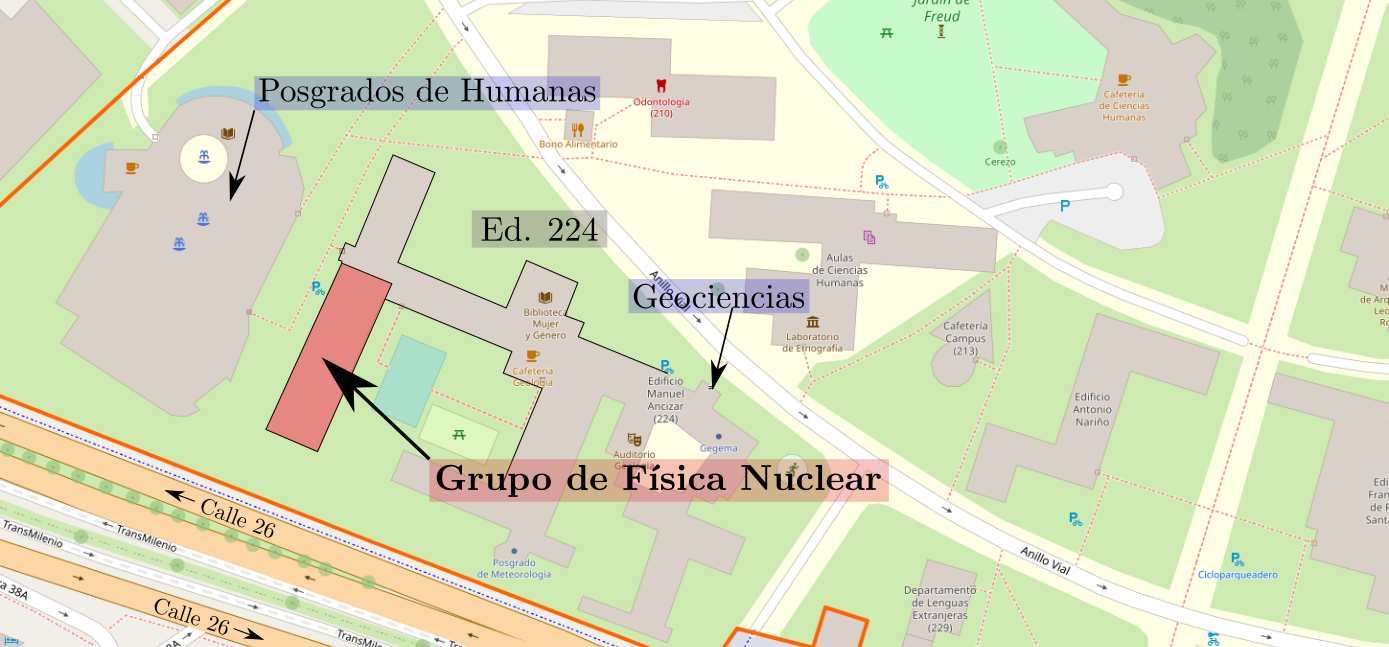
\includegraphics[height=4cm,  keepaspectratio]{Images/map2.png}
	\end{center}
\end{frame}

\begin{frame}{Presentación y Objetivos del Curso}
	\vspace{-0.3cm}
	\begin{columns}[T] 
		
		\begin{column}{0.55\textwidth}
			\textbf{¿Por qué Física en Biociencias?}
			\vspace{0.2cm}
			\begin{itemize}
				\item \textbf{Comprensión Cuantitativa:} Utilizar la mecánica clásica para modelar y entender fenómenos de sistemas vivos.
				\vspace{0.15cm}
				\item \textbf{Criterio Experimental:} Desarrollar destreza en la toma de datos, instrumentación e incertidumbres.
				\vspace{0.15cm}
				\item \textbf{Aplicación Práctica:} Conectar leyes físicas con la biomecánica, fisiología, agronomía y ciencias del suelo.
			\end{itemize}
		\end{column}
		
		\begin{column}{0.42\textwidth}
			\centering
			
\includegraphics[width=\linewidth, height=0.65\paperheight, keepaspectratio]{Images/meme1.jpeg}
		\end{column}
	\end{columns}
\end{frame}

    % ----- SLIDE 3: METODOLOGÍA -----
    \begin{frame}{Estructura de la Sesión (2 Horas)}
        \begin{block}{Distribución orientativa del tiempo}
            \begin{itemize}
                \item \textbf{15 min -- Quiz y Contexto:} Evaluación corta de lectura previa e introducción.
                \item \textbf{75 min -- Montaje y Mediciones:} Toma de datos experimentales con sensores o equipos.
                \item \textbf{30 min -- Procesamiento y Cierre:} Análisis inicial de datos y revisión de bitácora.
            \end{itemize}
        \end{block}
        
        \vspace{0.2cm}
        \centering
        \small \textit{"La toma de datos y su análisis inmediato son un solo proceso inseparable."}
    \end{frame}

    % ----- SLIDE 4: EVALUACIÓN ([shrink] para ajustar tabla y texto) -----
\begin{frame}{Sistema de Evaluación}
	\vspace{-0.2cm}
	\begin{columns}[T]
		\begin{column}{0.38\textwidth}
			\centering
			\renewcommand{\arraystretch}{1.3}
			\begin{tabular}{@{}lc@{}}
				\toprule
				\textbf{Componente} & \textbf{\%} \\
				\midrule
				Talleres (individual) & 10\% \\
				Bitácoras (grupal)    & 50\% \\
				Informes (grupal)     & 30\% \\
				Quices (individual)   & 10\% \\
				\midrule
				\textbf{Total} & \textbf{100\%} \\
				\bottomrule
			\end{tabular}
			
			\vspace{0.3cm}
			{\small \textcolor{gray}{Asistencia mínima: 80\%}}
		\end{column}
		
		\begin{column}{0.58\textwidth}
			\small
			\begin{description}
				\item[Talleres (2)] Fundamentación individual: cifras significativas, errores, incertidumbres y gráficos.
				\vspace{0.15cm}
				\item[Bitácoras] Reporte grupal de prácticas: montaje, datos, gráficos, análisis y conclusiones. \textit{Sin marco teórico.}
				\vspace{0.15cm}
				\item[Informes (2)] Formato artículo académico: marco teórico, metodología, discusión y referencias.
				\vspace{0.15cm}
				\item[Quices] Lectura previa, al inicio de cada sesión.
			\end{description}
		\end{column}
	\end{columns}
\end{frame}

    % ----- SLIDE 5: PENALIZACIONES -----
\begin{frame}{Puntualidad y Entregas Tardías}
	\vspace{-0.2cm}
	\begin{columns}[T]
		\begin{column}{0.55\textwidth}
			\textbf{Quices}
			\vspace{0.1cm}
			
			\small
			\begin{itemize}
				\item Se aplican en los \textbf{primeros 15 min}.
				\vspace{0.15cm}
				\item \textbf{No} hay quices extemporáneos por llegada tarde.
			\end{itemize}
			
			\vspace{0.3cm}
			\textbf{Asistencia}
			\vspace{0.1cm}
			
			\small
			\begin{itemize}
				\item Mínimo \textbf{80\%} para habilitar la nota final.
			\end{itemize}
		\end{column}
		
		\begin{column}{0.44\textwidth}
			\textbf{Entregas Tardías (Classroom)}
			\vspace{0.1cm}
			
			\renewcommand{\arraystretch}{1.25}
			\begin{tabular}{lcc}
				\toprule
				\textbf{Retraso} & \textbf{Nota} \\
				\midrule
				En plazo & 5.0 \\
				$+24$ h (1 día) & 4.0 \\
				$+48$ h (2 días) & 3.0 \\
				$+72$ h (3 días) & 2.0 \\
				$+96$ h (4 días) & 1.0 \\
				$> 96$ h ($>$4 días) & 0.0 \\
				\bottomrule
			\end{tabular}
		\end{column}
	\end{columns}
\end{frame}

% ----- SLIDE 6: BITÁCORA -----
% ----- SLIDE 6: BITÁCORA -----
\begin{frame}{El Cuaderno de Bitácora}
	\vspace{-0.3cm}
	\small
	\begin{itemize}
		\item \textbf{Formato:} Físico (cuaderno cuadriculado) o digital (Word, Google Sheets, \LaTeX). 
		Se recomienda el cuaderno físico para toma de datos en laboratorio y bosquejos iniciales.
		\vspace{0.08cm}
		\item \textbf{Antes del lab:} Responder preguntas previas de la guía. \textbf{No son calificables}, pero altamente recomendadas: de ellas salen los \textbf{quices}.
		\vspace{0.08cm}
		\item \textbf{En el lab:} Anotar procedimiento resumido, tablas de datos con \textbf{incertidumbres} y \textbf{unidades}. 
		\textcolor{red}{Sin incertidumbres o unidades en el entregable, la nota se reduce.}
		\vspace{0.08cm}
		\item \textbf{Gráficas:} Preliminares a mano, trazadas en clase para verificar tendencias. No busque perfección estética, busque claridad.
		\vspace{0.08cm}
		\item \textbf{Después del lab:} Redactar respuestas y análisis con buena ortografía y redacción. Numerar páginas/secciones para referencias cruzadas.
	\end{itemize}
\end{frame}

% ----- SLIDE: ACTIVIDAD INTRODUCTORIA -----

% ----- SLIDE: ACTIVIDAD INTRODUCTORIA -----
\begin{frame}{Actividad Flash: Frecuencia Cardíaca}
	\begin{columns}[T]
		\begin{column}{0.50\textwidth}
			\textbf{Instrucciones:}
			\begin{enumerate}
				\item Siéntate en silencio, con la espalda recta.
				\item Ubica tu pulso \textbf{radial} (muñeca) o \textbf{carotídeo} (cuello).
				\item Cierra los ojos y concéntrate en sentir los latidos.
				\item Al escuchar el "Start", cuenta en silencio los latidos durante \textbf{30 segundos}.
				\item Anota tu número de latidos $N$.
				\item Repite una segunda vez para comparar.
			\end{enumerate}
		\end{column}
		\begin{column}{0.46\textwidth}
			\centering
			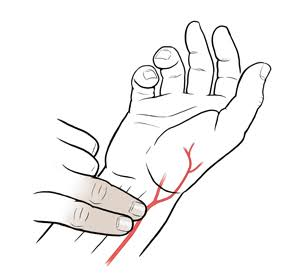
\includegraphics[width=\linewidth, height=0.6\paperheight, keepaspectratio]{Images/pulso.jpeg}
			\vspace{0.1cm}
		\end{column}
	\end{columns}
\end{frame}

\begin{frame}{Actividad Flash: Cálculo y Reflexión}
	\vspace{-0.2cm}
	\begin{block}{Conversión a bpm}
		\centering
		\Large
		$f = 2 \times N$ \hspace{0.5cm} [latidos por minuto]
	\end{block}
	
	\vspace{0.1cm}
	\textbf{Ejemplo:} Si contaste $N=22$ latidos en 30 s → $f = 2 \times 22 = 44$ bpm.
	
	\vspace{0.15cm}
	\textbf{Preguntas para reflexionar (en grupo):}
	\begin{itemize}
		\item ¿Cuál crees que es la incertidumbre $\Delta N$ de tu conteo? ¿Por qué?
		\item Si multiplicaste por 2, ¿cómo crees que afecta eso a la incertidumbre final?
		\item ¿Todos obtuvieron el mismo resultado? ¿Debería ser así?
	\end{itemize}
	
	\vspace{0.15cm}
	\centering
	\textcolor{blue}{\textbf{Guardemos esos datos... ¡vamos al tablero!}}
\end{frame}

\begin{frame}{Actividad Flash: Construyamos el Histograma}
	\vspace{-0.2cm}
	\begin{columns}[T]
		\begin{column}{0.54\textwidth}
			\textbf{Instrucciones (2 Mediciones):}
			\vspace{0.1cm}
			\begin{enumerate}
				\item Toma dos Post-its (Medición 1 y Medición 2).
				\item Usa tus dos valores de $N$ (los que anotaste antes).
				\item Calcula para cada uno: $f = 2 \times N$ [bpm].
				\item Escribe UNA frecuencia por Post-it.
				\item Pasa al tablero y ubica cada Post-it en su rango, \textbf{uno encima del otro}.
			\end{enumerate}
		\end{column}
		
		\begin{column}{0.44\textwidth}
			\begin{block}{Rangos en el Tablero [bpm]}
				\centering
				\small
				\vspace{0.1cm}
				$54-56$ \hspace{0.3cm} $57-59$ \\
				\vspace{0.1cm}
				$60-62$ \hspace{0.3cm} $63-65$ \\
				\vspace{0.1cm}
				$66-68$ \hspace{0.3cm} $69-71$ \\
				\vspace{0.1cm}
				$72-74$ \hspace{0.3cm} $\ge 75$
				\vspace{0.1cm}
			\end{block}
		\end{column}
	\end{columns}
\end{frame}

\begin{frame}{Actividad Flash: Discusión Final}
	\vspace{-0.2cm}
	\textbf{Miremos el histograma:}
	\begin{itemize}
		\item ¿Ven una forma de \textbf{campana}? 
		\item ¿La dispersión se debe a errores de medición o a diferencias reales entre personas?
		\item Según lo que discutimos, ¿cuál crees que es la incertidumbre $\Delta f$?
	\end{itemize}
	
	\vspace{0.15cm}
	\textbf{Conceptos clave:}
	\begin{description}
		\item[Variabilidad biológica:] Los seres vivos son diferentes por naturaleza.
		\item[Error aleatorio:] Dificultad de contar latidos en 30 s exactos.
		\item[Sesgo sistemático:] ¿Alguien tomó café? ¿Corrió para llegar?
	\end{description}
	
	\vspace{0.15cm}
	\centering
	\textcolor{red}{\textbf{¿Qué tipo de error domina en nuestro histograma?}}
\end{frame}

\begin{frame}{Próximos Pasos para la Semana 2}
	\begin{columns}[T]
		\begin{column}{0.55\textwidth}
			\begin{block}{Para la siguiente sesión (08/09):}
				\begin{itemize}
					\item Consultar el enlace del cronograma fijado en Classroom.
					\item Conformar los grupos de trabajo (3 a 4 personas).
					\item Revisar el material sobre incertidumbres experimentales para el \textbf{Taller 1}.
				\end{itemize}
			\end{block}

		\end{column}
		
		\begin{column}{0.40\textwidth}
			\centering
			
\includegraphics[width=\linewidth, height=0.7\paperheight, keepaspectratio]{Images/meme2.jpeg}
		\end{column}
	\end{columns}
\end{frame}

\end{document}